\section{Results}
\label{sec:results}

In order to answer the posted research questions, the results from the aforementioned analyses are described in this section.

\subsection{Simple comparisons}

In this section, the results from simple two-sample comparisons between the two cohorts are presented. Each type of aggregation is shown separately.

\subsubsection{Overall aggregated measures}

To assess baseline differences in affective expression between clinical groups, we first examined overall NA levels and their variability across the entire time series. A Mann-Whitney U test confirmed a significant difference in mean NA levels between the depression and anxiety cohorts ($U = 227445$, $p < .001$). Individuals diagnosed with depression exhibited higher average NA levels ($M = 0.0878$) compared to those in the anxiety cohort ($M = 0.0844$). This result suggests that, on average, individuals with depression report more pronounced negative affect throughout the study period than those with anxiety.

In addition to absolute NA levels, we also investigated the variability of negative affect, operationalized as the standard deviation of NA scores across the full time series for each individual. Again, a significant difference was observed ($U = 237172$, $p < .001$), with the depression cohort displaying greater affective instability. Specifically, the mean standard deviation of NA scores was $0.1356$ in the depression cohort, compared to $0.1276$ in the anxiety cohort. This finding suggests that individuals with depression not only experience more intense negative affect but also exhibit more fluctuations in their emotional state over time.

These results, visualized in Figure \ref{fig:overall_histograms}, provide strong evidence that depression is associated with both higher levels and greater variability of negative affect when examined across the entire observational window. 



\begin{figure}[h]
    \centering
    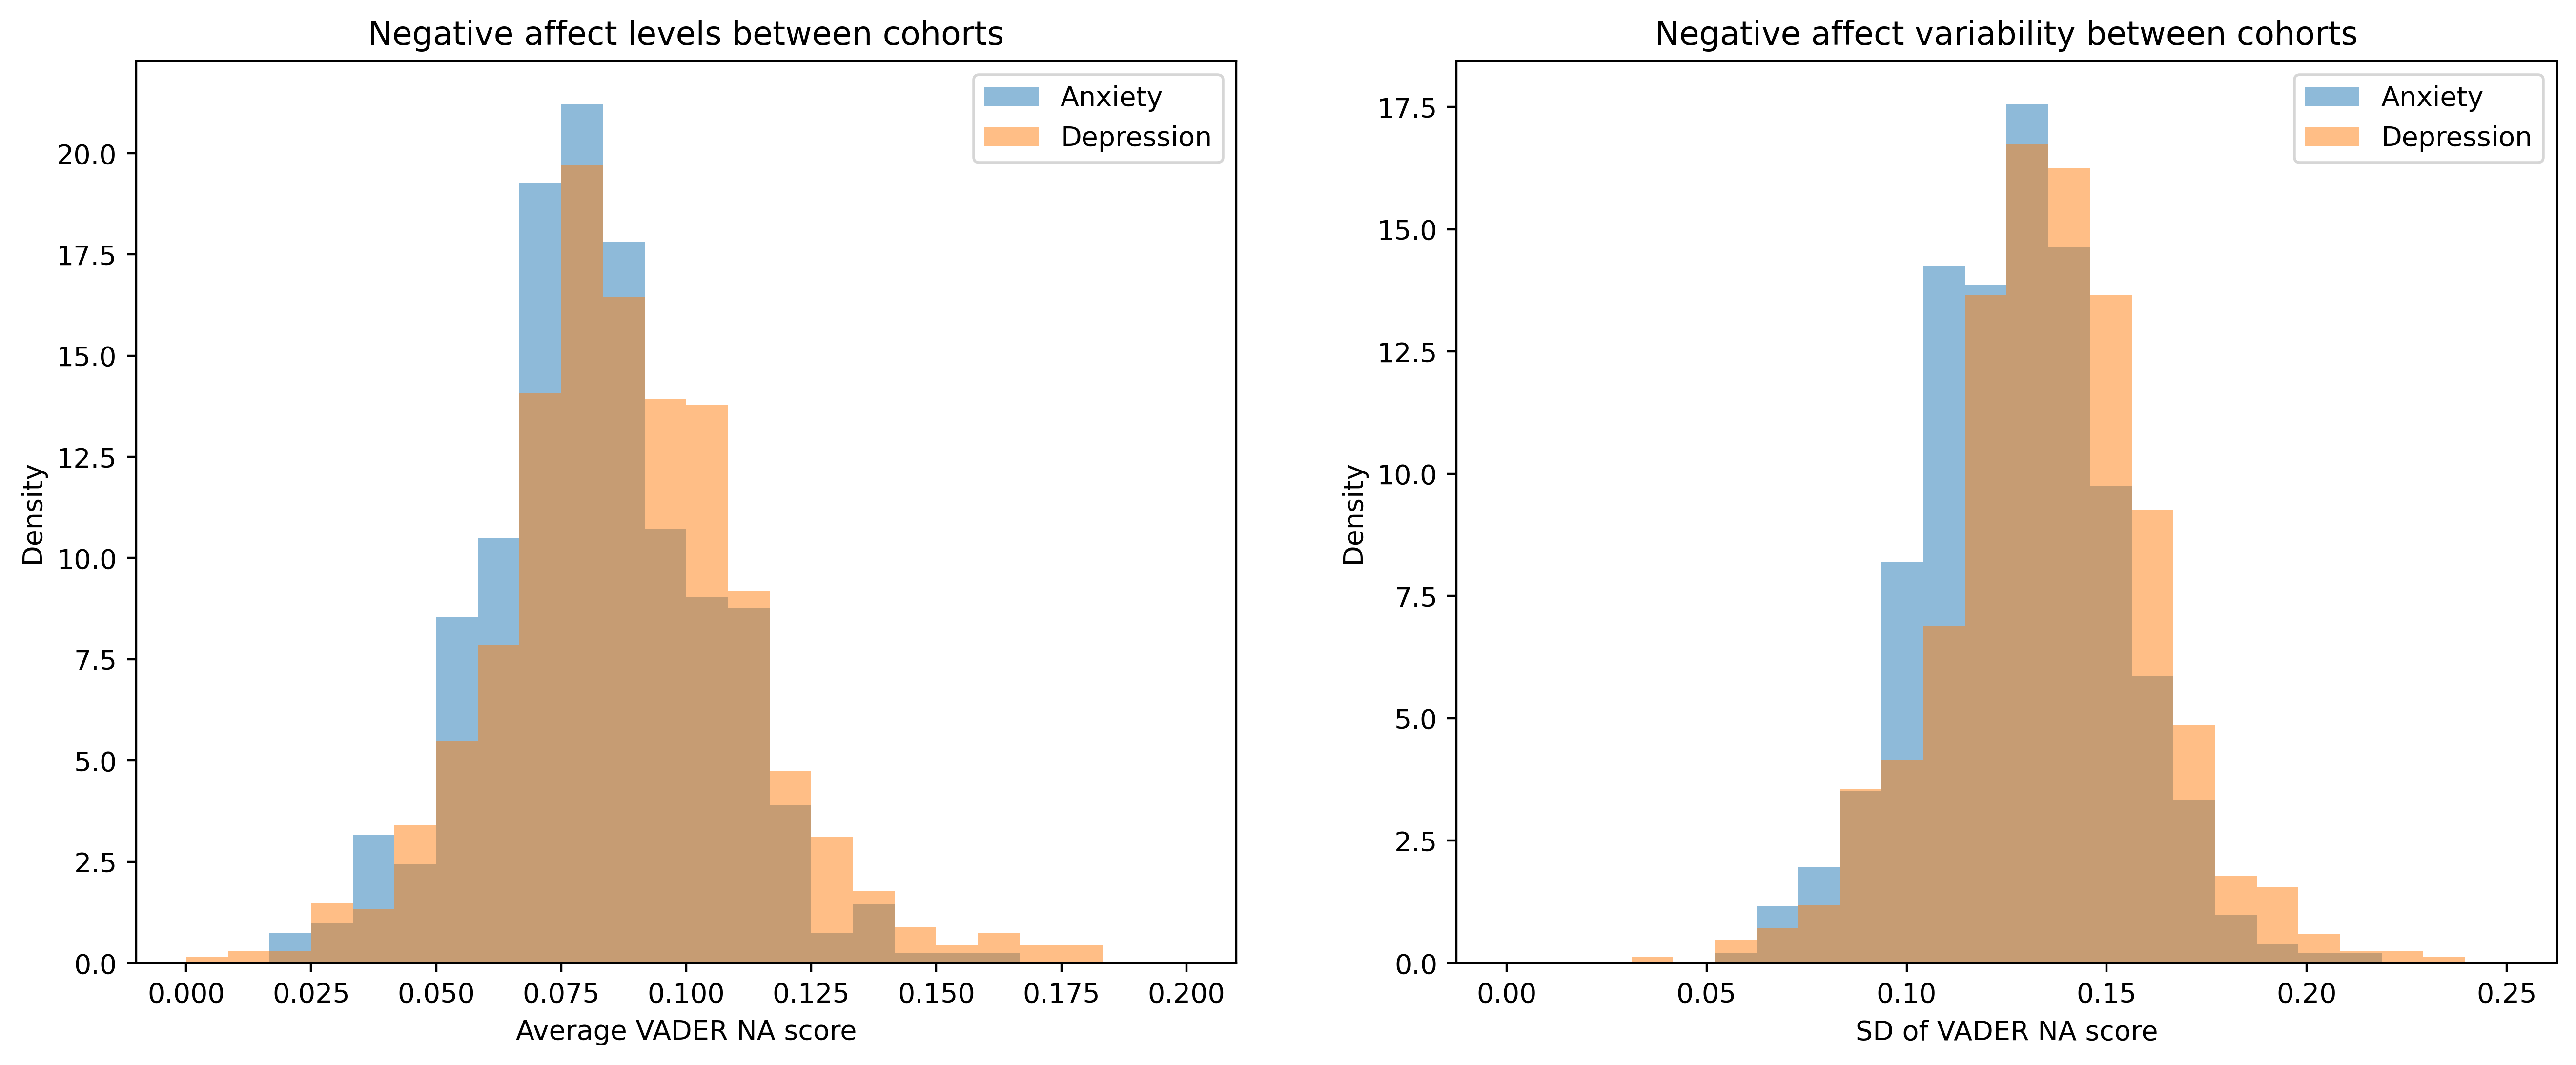
\includegraphics[width=\linewidth]{Images/na_histograms_overall.png}
    \caption{Negative affect level and spread across the entire time series, grouped by cohort.}
    \label{fig:overall_histograms}
\end{figure}

\subsubsection{6-hour windows}

%Moved to different section:
%Before interpreting the results obtained from the 6-hour window approach, it is crucial to assess whether the arithmetic mean and standard deviation serve as appropriate summary statistics for aggregating negative affect (NA) levels and their variability across individuals. If these measures fail to accurately represent the underlying distributions, subsequent inferences may be biased or misleading.

%To evaluate this assumption, the distributions of aggregated values for each subject are examined by comparing their means and medians. A significant difference between these measures would suggest that the data is skewed or contains outliers, potentially violating the assumption that the arithmetic mean is a robust central tendency measure. In the case of negative affect levels, computed as the mean across all 6-hour windows per subject, this assumption does not hold ($U = 1820498$, $p < .001$), indicating that the mean may not adequately summarize the distribution of NA levels.

%A similar issue is observed for negative affect variability, measured as the standard deviation across all 6-hour windows per subject. The significant test result ($U = 2187117.5$, $p < .001$) suggests that the standard deviation may not be the most reliable measure of variability, which requires careful interpretation of subsequent analyses.

\begin{figure}[h]
    \centering
    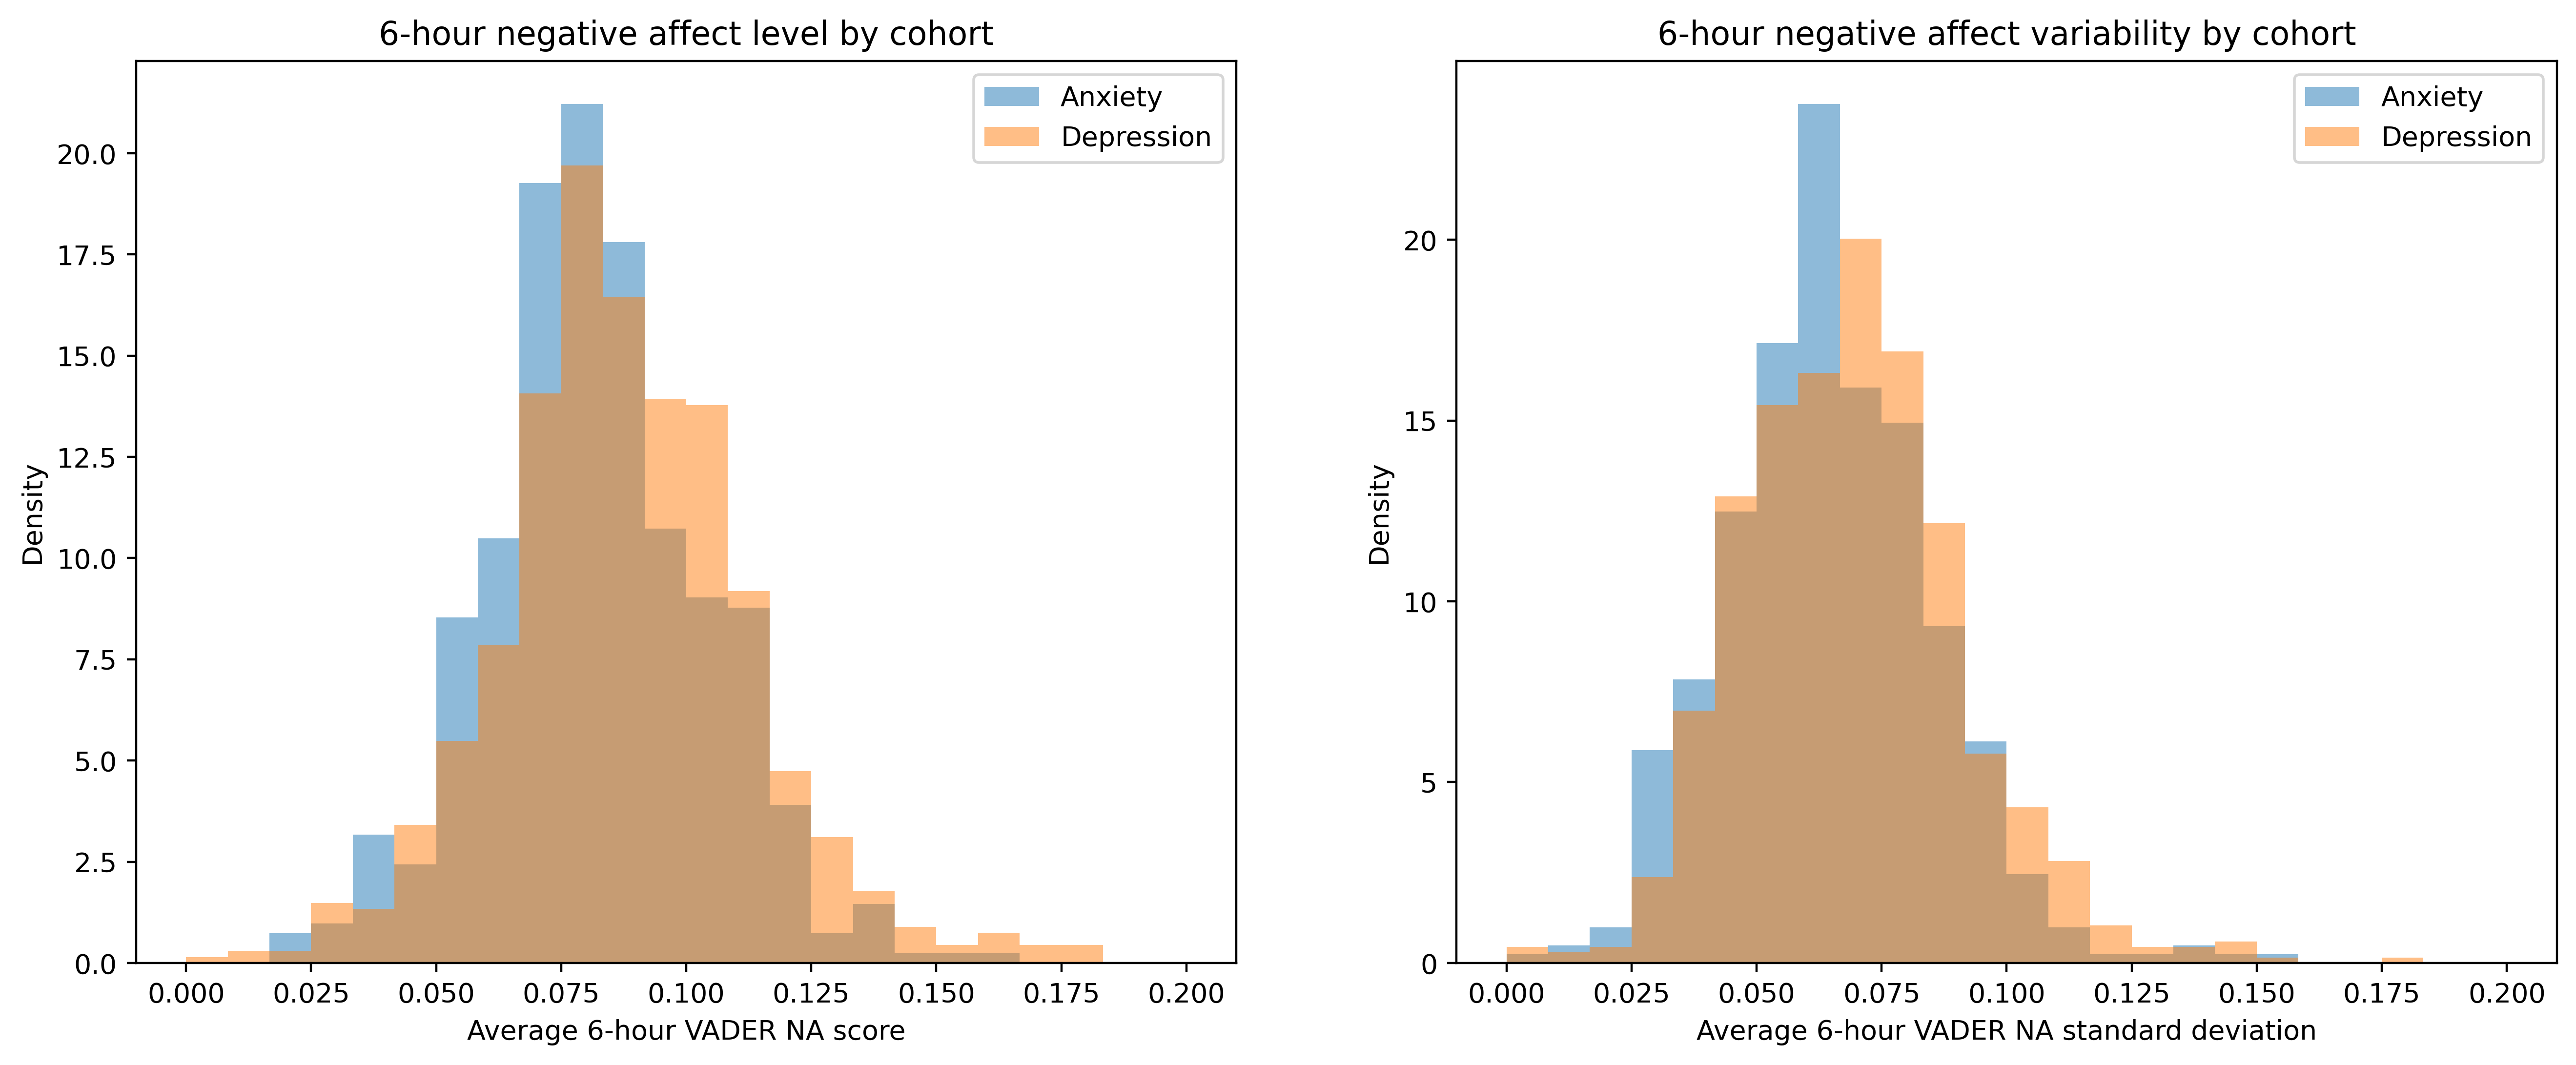
\includegraphics[width=\linewidth]{Images/na_histograms_6hr.png}
    \caption{Negative affect level and spread during 6-hour windows, grouped by cohort.}
    \label{fig:6hr_histograms}
\end{figure}

Figure \ref{fig:6hr_histograms} presents the distributions of negative affect levels and variabilities across subjects. Consistent with previous findings, the depression cohort had significantly higher NA levels than the anxiety cohort. Specifically, the mean NA level for the depression cohort was 0.0881, compared to 0.0823 in the anxiety cohort ($U = 636510$, $p < .001$). This result reinforces the distinction between the two clinical groups, with individuals diagnosed with depression expressing more pronounced negative affect.

Beyond differences in absolute NA levels, the depression cohort also demonstrated significantly greater variability in negative affect, with a mean variability of 0.0693 compared to 0.0648 in the anxiety cohort ($U = 1050891$, $p < .001$). This finding suggests that individuals with depression not only experience heightened negative affect but also exhibit more unstable affective patterns over time.

\subsubsection{Daily aggregation}

With each person's daily NA level fluctuations reduced to a single average value, the distributions as shown in Figure~\ref{fig:daily_histograms} emerged. Again, the depression cohort showed significantly higher NA levels than the anxiety cohort. Specifically, the mean NA level for the depression cohort was $0.0873$, compared to $0.0822$ in the anxiety cohort ($U = 222435$, $p < .001$). This result agrees with the previous finding.

Furthermore, the depression cohort exhibited significantly greater variability in negative affect, with a mean variability of $0.0885$ compared to $0.0809$ in the anxiety cohort ($U = 224679$, $p < .001$). This also supports the results from the 6-hour windows and indicates that NA variability is lower for the A cohort than the D cohort, supporting the hypothesized differences according to the CAM.

\begin{figure}[h]
    \centering
    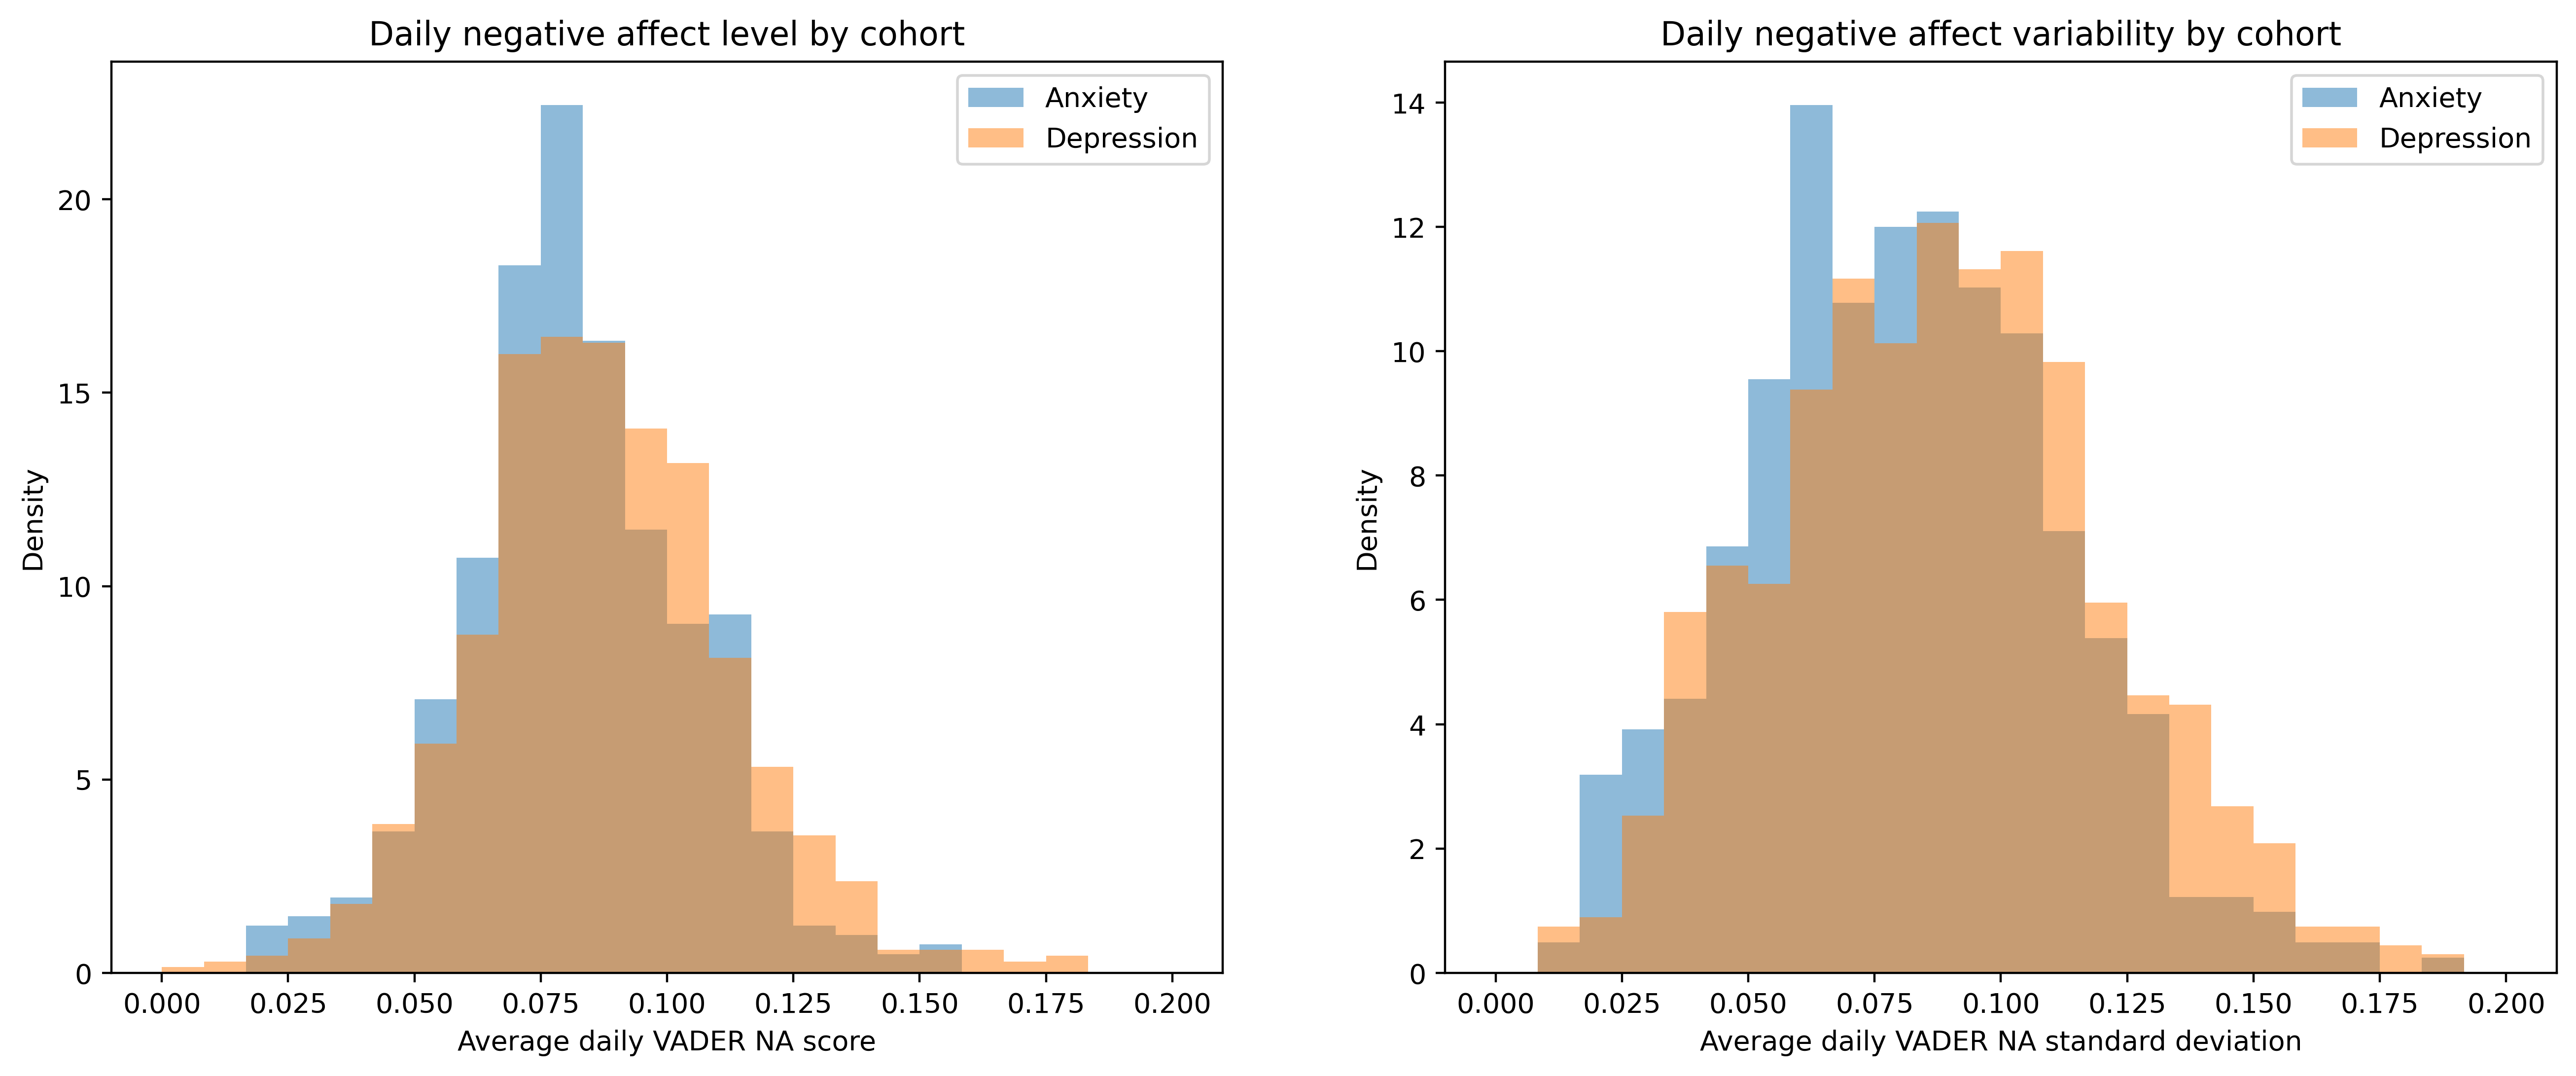
\includegraphics[width=\linewidth]{Images/na_histograms_daily.png}
    \caption{Negative affect level and spread during daily windows, grouped by cohort.}
    \label{fig:daily_histograms}
\end{figure}


\subsection{LMM}

In this section, the results for the linear mixed model approach are presented. First, results for tweet-level sentiments are shown, then for 6-hour aggregations.

\subsubsection{No aggregation}

Fitting the LMM to the whole dataset, the optimal spline knot placement according to RMSE was three knots with a polynomial degree of two, placed at 6 AM, 12 AM and 6 PM.

The spline plot, shown in Figure~\ref{fig:spline_preds_raw}, shows how NA levels were relatively stable throughout the day, with a pronounced peak in the afternoon, between 1 PM and 5 PM.

\begin{figure}[h]
    \centering
    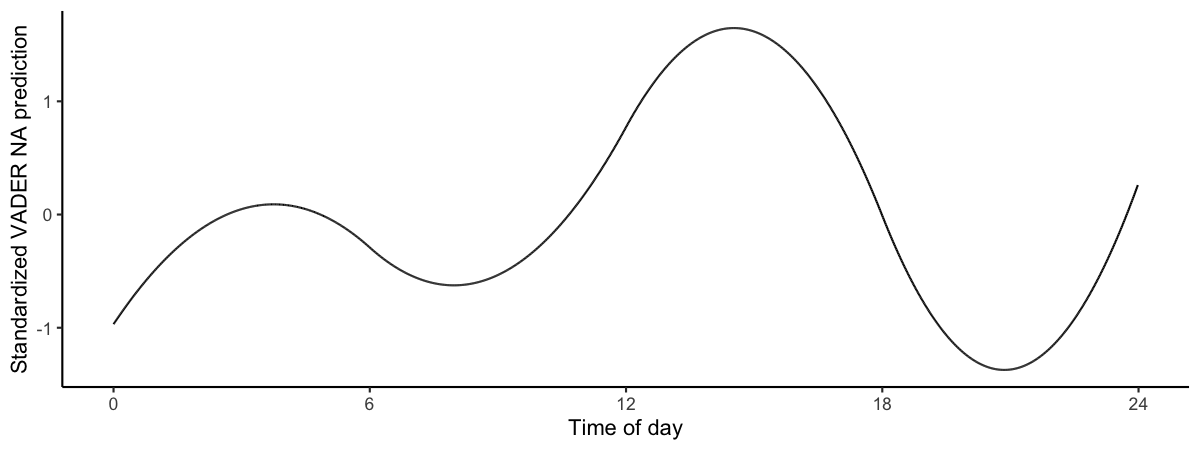
\includegraphics[width=\linewidth]{Images/lmm_raw_spline.png}
    \caption{Spline fit from LMM on tweet-level VADER-based sentiment data.}
    \label{fig:spline_preds_raw}
\end{figure}

The model represented a very weak fit, indicated by conditional $R^2$ of $0.03$. This was likely due to the large amount of single tweets and heterogeneous NA levels when not applying any smoothing function.

The model revealed a strong positive autocorrelation in the VADER NA scores, with a significant regression coefficient for the previous NA score ($B = 0.0488; p < .001$), suggesting that individuals' current NA levels are influenced by their previous NA levels, highlighting temporal dependence in emotional expression.

The time between consecutive tweets did not have a significant impact on NA scores ($B = -0.00005; p = .29$), indicating that the timing or duration between social media posts does not notably affect participants' NA levels, suggesting that posting frequency is not a strong predictor of emotional changes.

Although NA levels tended to be slightly higher on weekends, the difference was not statistically significant ($B = 0.0005; p = .08$), suggesting that the observed weekend effect on NA levels may be due to random variation rather than a consistent pattern.

However, NA variability was significantly greater on weekends compared to weekdays ($F(1, 1130402) = 12.703; p < .001$), with a standard deviation of $0.136$ on weekends versus $0.135$ on weekdays. This indicates that, while NA levels themselves may not differ, there is greater fluctuation in emotional experiences over the weekend, possibly reflecting changes in mood or social interaction patterns.

No significant differences were found across age groups in NA levels, suggesting that age does not significantly impact the average level of negative affect experienced by participants in this study.

Additionally, there were no significant gender differences in NA levels ($B = 0.0007; p = .62$), indicating that men and women in this sample report similar average levels of negative affect, despite potential differences in emotional experiences or expression.

Women showed significantly lower NA variability ($F(1, 1130402) = 7.17; p = .007$), with a residual standard deviation of $0.134$, compared to $0.136$ for men. This suggests that women may experience more stable emotional states, with less fluctuation in their NA levels across time.

Participants in the A cohort exhibited significantly lower NA levels than participants in the D cohort ($B = -0.0054; p < .001$), indicating that individuals with anxiety generally report lower negative affect compared to those with depression, consistent with the clinical distinction between the two conditions.

\begin{figure}
    \centering
    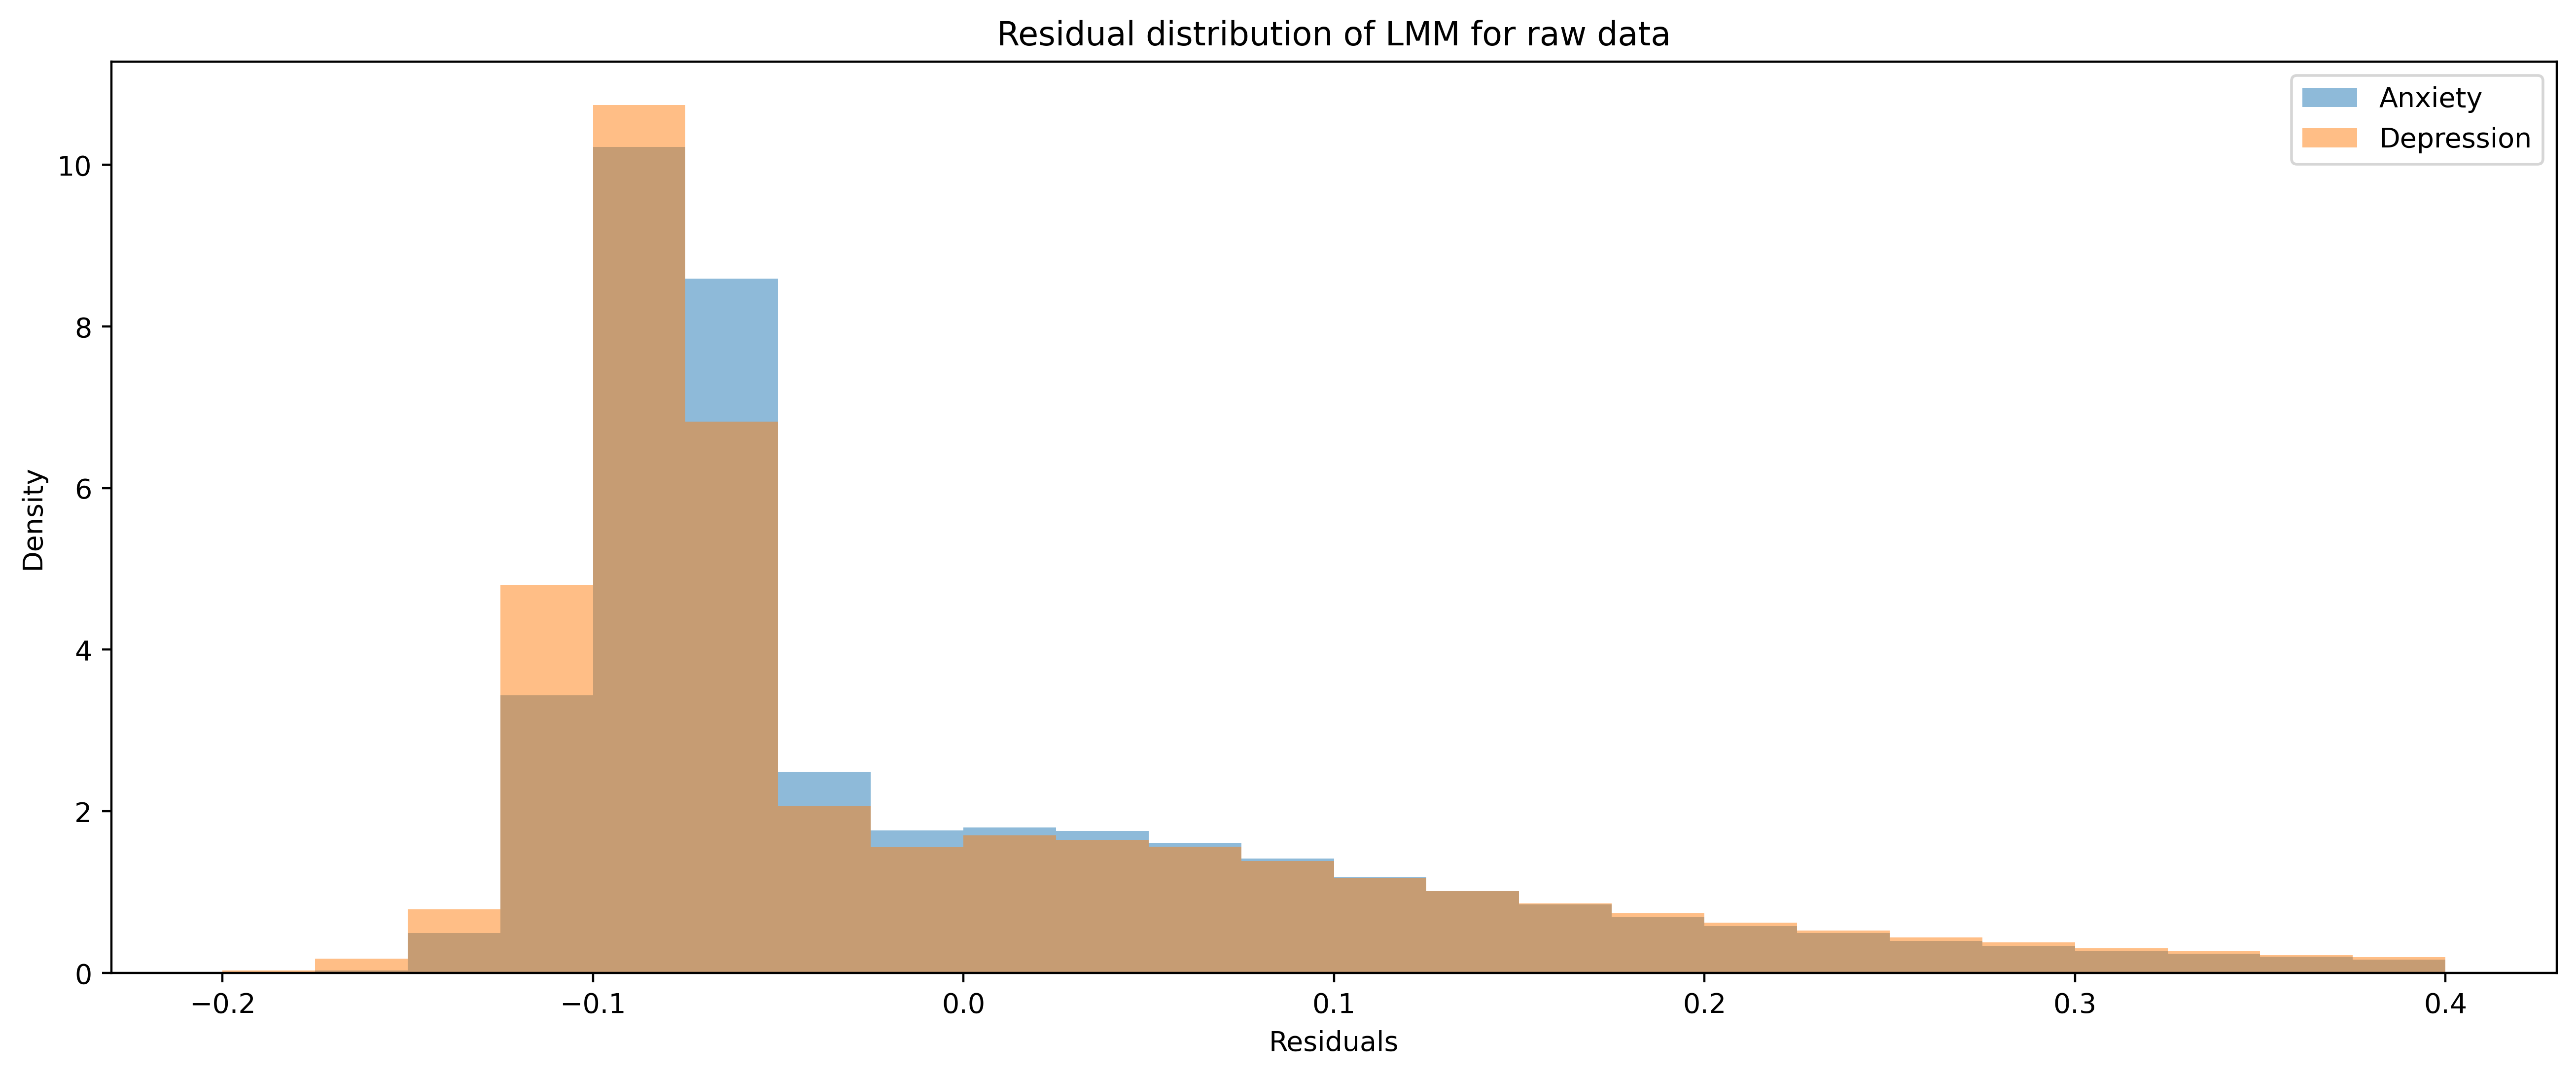
\includegraphics[width=\linewidth]{Images/lmm_raw_vader_residuals.png}
    \caption{Residual distribution by cohort for raw data LMM predictions}
    \label{fig:raw_lmm_hist}
\end{figure}

Furthermore, the A cohort showed lower NA variability (see Figure~\ref{fig:raw_lmm_hist}), with a residual standard deviation of $0.130$, compared to $0.138$ in the D cohort. This difference in variability was highly significant ($F(1, 1130402) = 713.84; p < .001$), suggesting that depression patients experience greater fluctuations in negative affect, potentially reflecting the emotional instability often associated with depressive disorders.

\subsubsection{6-hour windows}

Using 6-hour aggregated data, the optimal placement of spline knots was determined to be four equidistant knots placed throughout the day, with a polynomial degree of three. This configuration provided a balance between flexibility and parsimony, allowing the model to capture meaningful fluctuations in NA levels without overfitting to short-term variations.

The resulting spline fit is illustrated in Figure \ref{fig:spline_preds_6hr}. The fitted curve reveals a distinct increase in NA levels around 4 AM, suggesting an increase in engagement with emotionally negative content during the early morning hours. Following this rise, NA levels remain relatively stable throughout the rest of the day, with no pronounced peaks or troughs.

\begin{figure}[h]
    \centering
    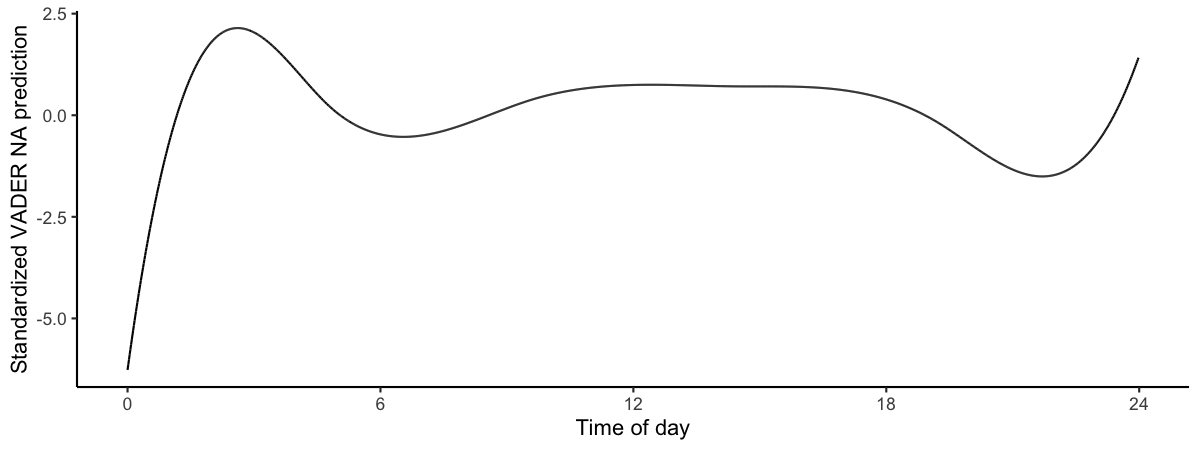
\includegraphics[width=\linewidth]{Images/lmm_6hr_spline.png}
    \caption{Spline fit from LMM on 6-hour windowed VADER-based sentiment data.}
    \label{fig:spline_preds_6hr}
\end{figure}

The model demonstrated a good fit, with an explained variance of $R^2 = 0.51$ as measured by conditional $R^2$. While this suggests that a significant portion of the variance in NA levels can be accounted for by the predictors included, a substantial proportion remains unexplained, likely due to unmeasured individual differences or external contextual factors.

The previous (autoregressive) VADER NA score exhibited a strong positive association with the current NA score ($b = 0.69$, $p < .001$), indicating that an individual's emotional state is highly correlated across consecutive tweets. This suggests a degree of temporal stability in NA levels, wherein prior emotional states strongly influence subsequent affective expression.

In contrast, the time elapsed between tweets did not show a statistically significant relationship with NA levels ($b = -0.000004$, $p = .85$). This suggests that the passage of time alone is not a meaningful predictor of fluctuations in expressed negative affect, at least within the timeframes typically observed in social media activity.

Tweets posted on weekends differed significantly in NA levels compared to those posted on weekdays ($b = 0.0002$, $p = .23$). This indicates that, on average, individuals express lower levels of negative affect throughout the week, with notable fluctuations between workdays and leisure days. In addition to the mean levels, an important difference also emerges when considering the variability in NA scores.

Residual variance, as a measure of NA variability, differed significantly between weekday and weekend tweets ($F(1, 1116317) = 8.69$, $p = .003$). Specifically, tweets posted on weekdays exhibited greater residual variance, implying that NA expression becomes less predictable during these periods. This suggests that individuals may experience more erratic emotional states on weekdays, potentially due to less focus on social and personal experiences.

None of the categorical age features had a significant association with NA levels, indicating that there are no systematic differences in expressed negative affect across age groups. This suggests that, at least within the sampled population, age does not meaningfully influence the extent of negative emotional expression on social media.

Similarly, no significant difference in NA levels was observed between men and women ($b = 0.0002$, $p = .68$). This finding aligns with previous research suggesting that while gender differences exist in broader emotional regulation and coping strategies, they may not necessarily manifest in overall levels of expressed negative affect.

However, while mean NA levels did not differ between genders, the variability in NA levels was different for men than for women. Levene's test for homogeneity of variance revealed significantly higher residual variance for women ($F(1, 1116317) = 44.56$, $p < .001$), indicating greater fluctuations in negative affect over time. This suggests that while men and women may express similar levels of negative affect on average, women's affective states appear to be more dynamic and less stable over time.

Membership in the anxiety cohort was found to be negatively associated with NA levels ($b = -0.0017$, $p < .001$), suggesting that individuals diagnosed with anxiety tend to express lower levels of negative affect than those diagnosed with depression. This finding is consistent with prior research indicating that while both conditions involve dysregulated affect, depression is typically characterized by more persistent and severe negative emotional states.

Beyond differences in NA levels, the two cohorts also differed in the predictability of their negative affect expression. The residual variance for the anxiety cohort was $0.0472$, compared to $0.0480$ for the depression cohort. As shown in Figure \ref{fig:6hrlmm_cohort_hist}, this difference was statistically significant ($F(1, 1116317) = 67.59$, $p < .001$). These results indicate that individuals with depression not only experience higher average levels of NA but also exhibit greater fluctuations in their negative affective expression, making their emotional states less predictable compared to those in the anxiety cohort.



\begin{figure}[h]
    \centering
    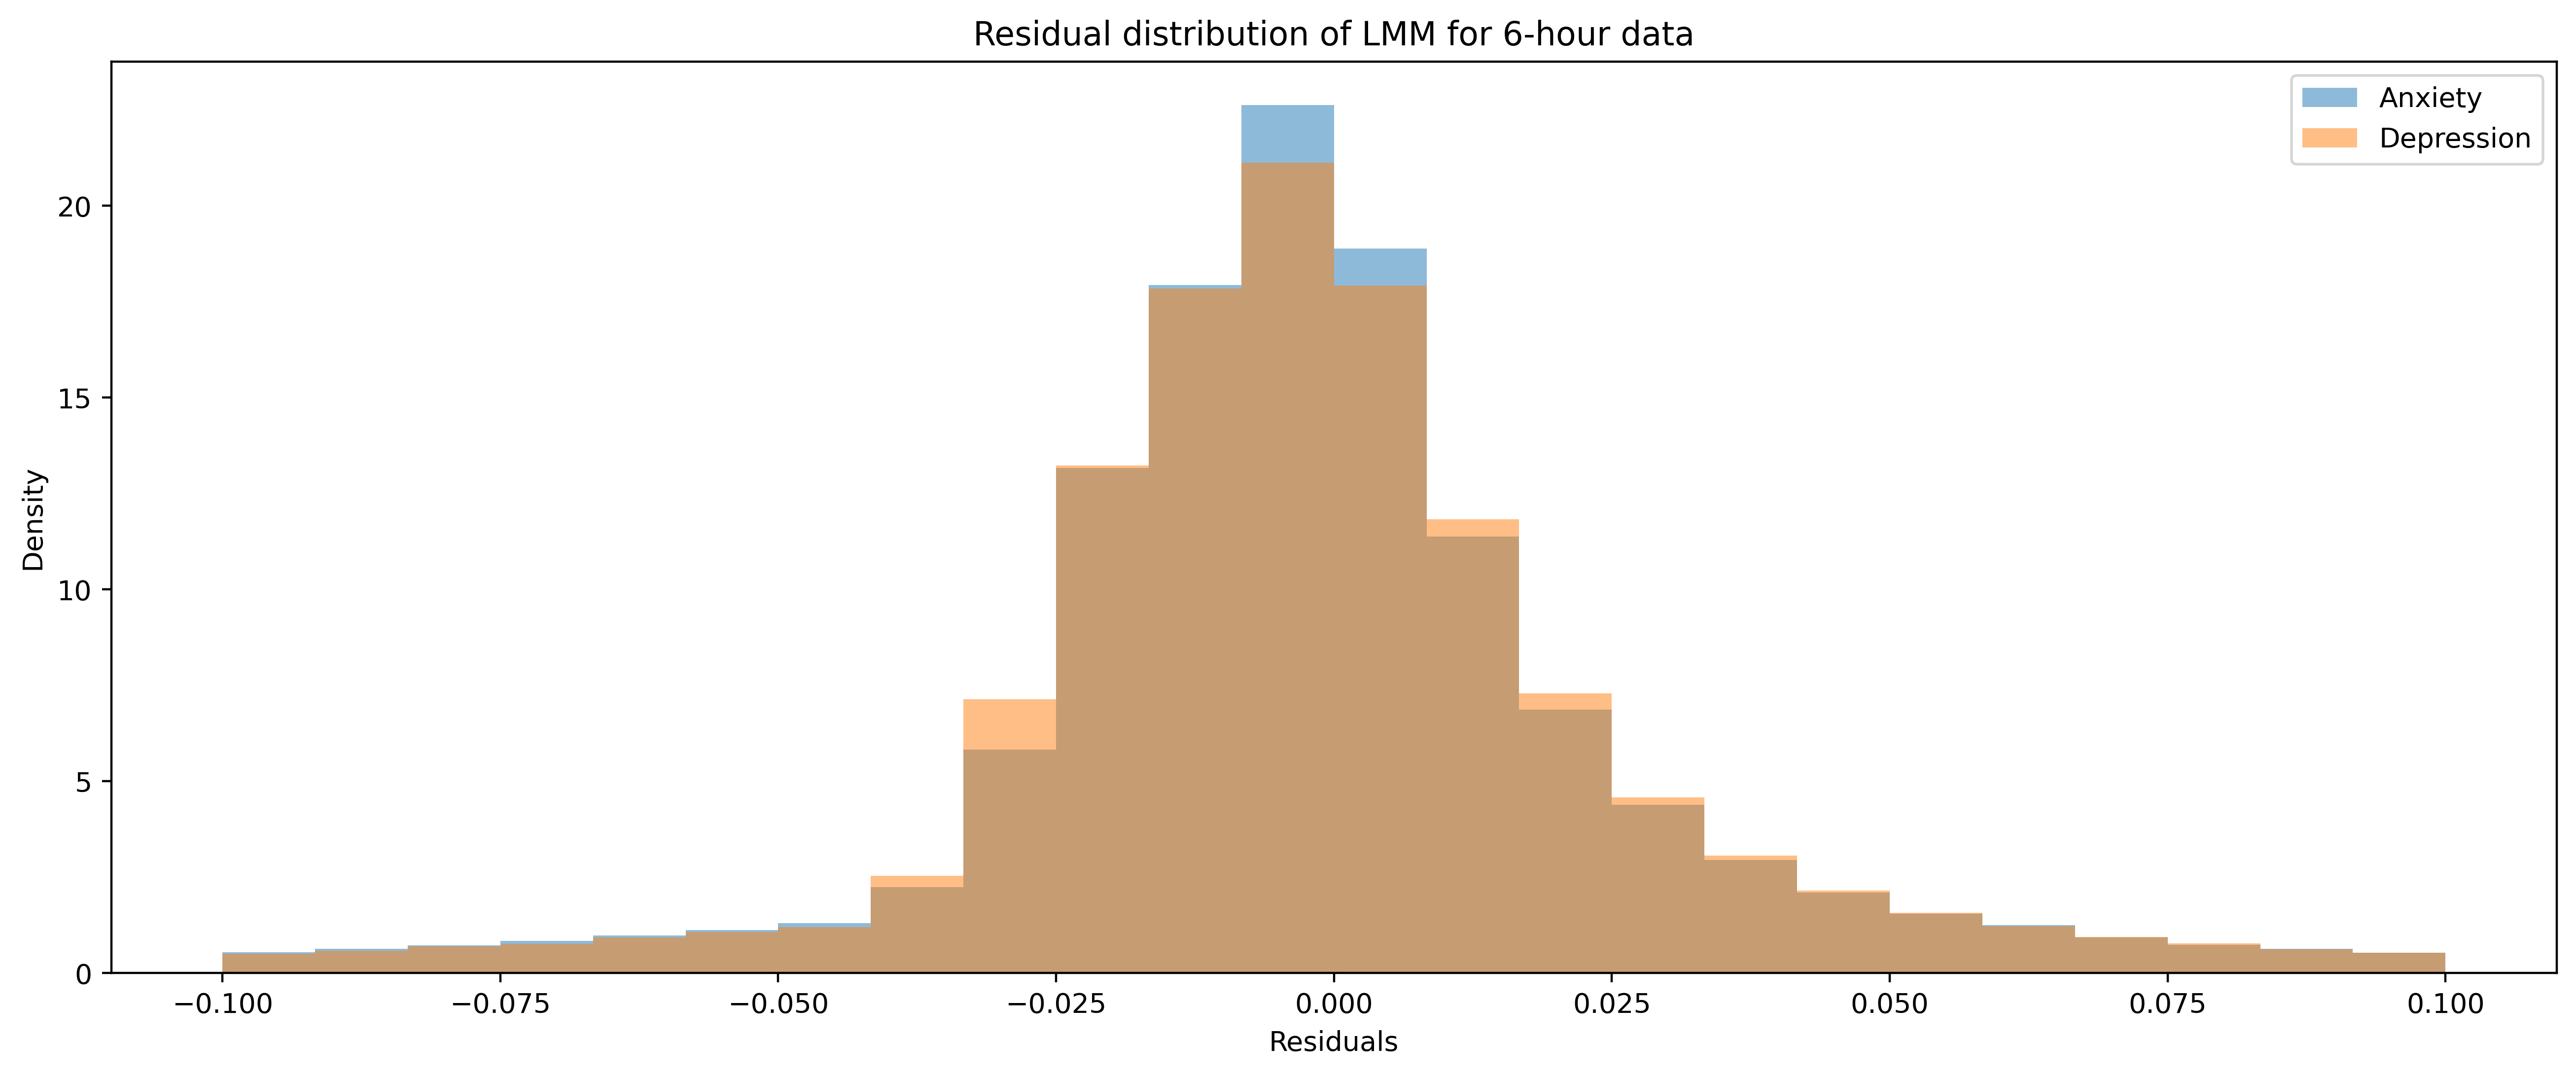
\includegraphics[width=\linewidth]{Images/lmm_6hr_vader_residuals.png}
    \caption{Residual distribution by cohort for 6-hour-windowed LMM predictions}
    \label{fig:6hrlmm_cohort_hist}
\end{figure}


\subsection{Robustness checks}

\subsubsection{Transformer-based analyses}

Prior to re-running the analyses based on RoBERTa-derived sentiment scores, the relationship between these scores and those obtained using the VADER approach was examined. Specifically, a Pearson correlation coefficient was calculated to assess the degree of linear association between the two sentiment measures across the full dataset. The resulting correlation coefficient was $r = 0.001$, indicating virtually no linear relationship between the VADER and RoBERTa sentiment scores. This lack of correlation suggests that the two methods capture fundamentally different aspects of sentiment within the data. Consequently, subsequent analyses based on RoBERTa scores may offer a distinct and potentially complementary perspective on the distribution of NA levels in the sample, independent of the VADER-based results.

As for the VADER-based analyses, the assumption of (approximate) symmetric NA level distributions was also checked for the RoBERTa scores. For the raw tweet-level data, the assumption did not hold since within-person mean and median are significantly different ($U = 167521; p < .001$). For the 6-hour windows, the assumption could not be rejected, since the means and medians of 6-hour window average scores for each person were not significantly different ($U = 113207; p = .07$). For daily aggregated data, again, the assumption did not hold ($U = 125065; p < .001$).

When applying the transformer-based sentiment analysis without any windowed aggregation — that is, based on raw, tweet-level sentiment estimates — significant differences in NA levels were observed between the A and D cohorts. Specifically, a Mann-Whitney U test indicated that NA levels differ significantly across groups ($U = 29385; p = .04$), with the average NA score being higher for the D cohort ($M = .2978$) compared to the A cohort ($M = .2792$). 

When examining NA variability, operationalized as the within-user standard deviation of NA scores, significant differences did not emerge between the two cohorts ($U = 27326; p = .58$). The D cohort again showed slightly higher average variability in NA ($M = .3196$) compared to the A cohort ($M = .3189$). Thus, the sample mean standard deviation was higher for the D cohort, although not statistically significant.

Similar results were found for the 6-hour aggregated data. The average NA level was higher in the D cohort with $.30$ compared to $.28$ for the A cohort ($U = 29364; p = .04$). There was no significant difference in NA variability though ($U = 26259; p = .89$). Descriptively, the A cohort showed slightly higher variability with a standard deviation of $.1789$ as compared to $.1786$ for the D cohort.

For daily aggregations, the D cohort again showed higher NA levels ($.29$) compared to the A cohort ($.27$), which was statistically significant ($U = 29318; p = .04$). The differences in NA variability were also not significant ($U = 26830; p = .79$), although the D cohort had slightly higher variability again ($.22$ compared to $.21$).

In addition to the overall differences, LMM was also fitted to the RoBERTa data.

The LMM showed substantial explanatory performance, with a conditional $R^2 = .59$. This indicates, that the model fit is quite good and the covariates in the model are able to explain a substantial amount of the variation in the RoBERTa NA scores.

The splines knots were optimally placed at 6AM, 12 AM and 6 PM, with a polynomial degree of two. The spline fit can be seen in Figure \ref{fig:roberta-spline}. NA levels were highest during the morning (6-12 AM) and appeared to be otherwise relatively stable throughout the day.

\begin{figure}[h]
    \centering
    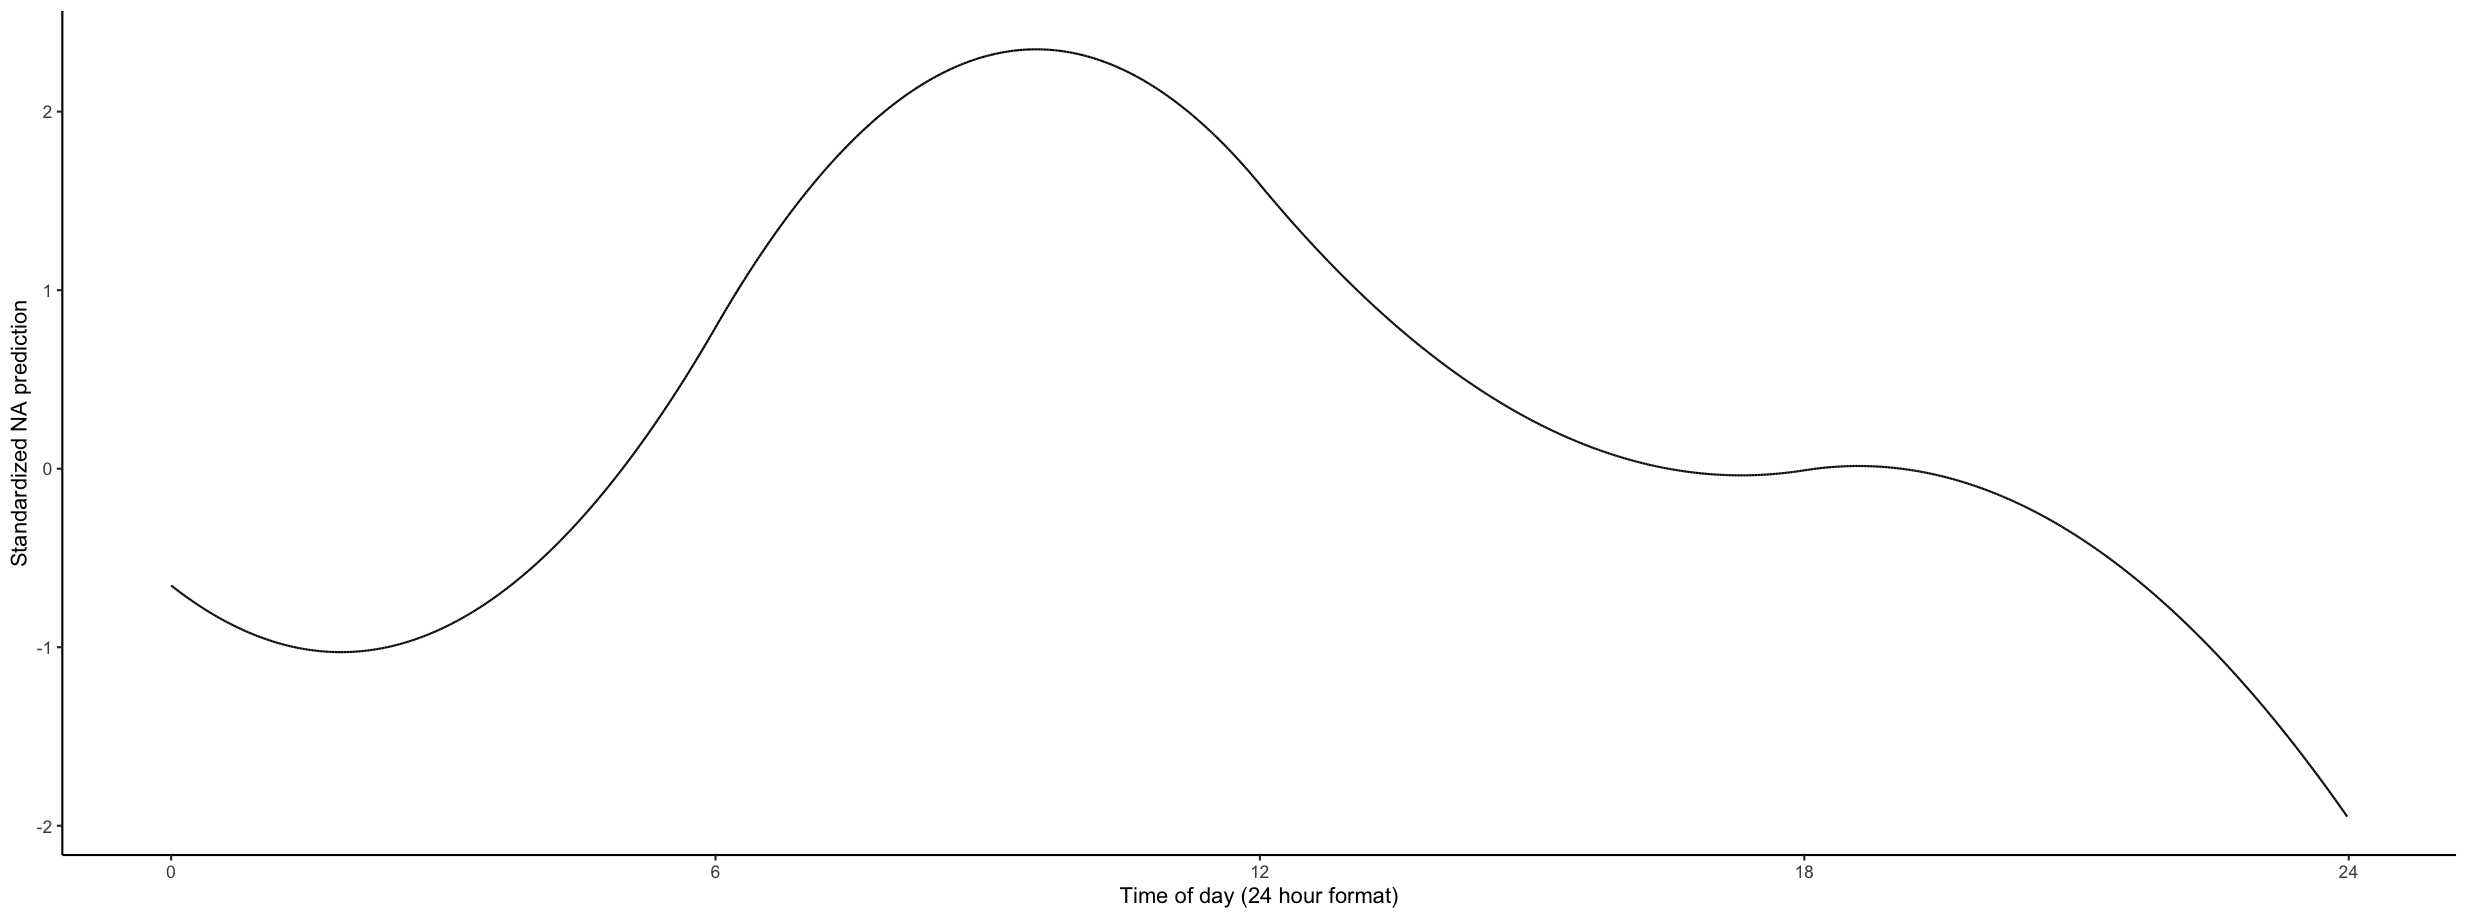
\includegraphics[width=\linewidth]{Images/roberta_lmm_splines.png}
    \caption{Spline fit from LMM on RoBERTa-based sentiment data of 250 sample participants.}
    \label{fig:roberta-spline}
\end{figure}

There was no difference between the genders regarding NA levels ($B = 0.0023; p = .45$) or the NA variability ($F(1, 279790) = 0.00; p = .99)$. Strong autocorrelation could still be observed between consecutive tweets ($B = 0.71; p < .001$). This indicates, that the baseline NA level for a 6-hour period is always offset by roughly $71\%$ of the NA level of the previous period.

NA levels were significantly lower on week ends ($B = -0.0009; p = .04$), indicating that users show less negative emotion online during the week ends.

%In the RoBERTa-based LMM, a statistically significant effect of the logarithmic time passed since the previous tweet could be observed ($B = -0.0012; p < .001$), indicating that NA levels tend to decrease over time when not actively posting on Twitter. More specifically, the point estimate suggests, that NA levels decline by $0.0012$ when multiplying the expired time by $e \approx 2.718$.

Using the RoBERTa NA scores as outcome variable, the anxiety cohort exhibited a higher NA variability as measured by residual standard deviation ($\sigma^2_A  = 0.123$) than the D cohort ($\sigma^2_D = 0.121$). This difference is statistically significant ($F(1, 407101) = 10.59; p = .001$). In order to further underline this finding, a nonparametric bootstrap procedure was run to compute confidence intervals for the difference in variability between the cohorts. In 1000 bootstrap replications, the 95 \% CI for the difference in variances is $[0.0007,  0.0030]$, further underlining, that the anxiety cohort showed higher residual variance and therefore higher NA variability. See Figure~\ref{fig:roberta-lmm-residuals} for a graphical representation of the residual distribution.

\begin{figure}
    \centering
    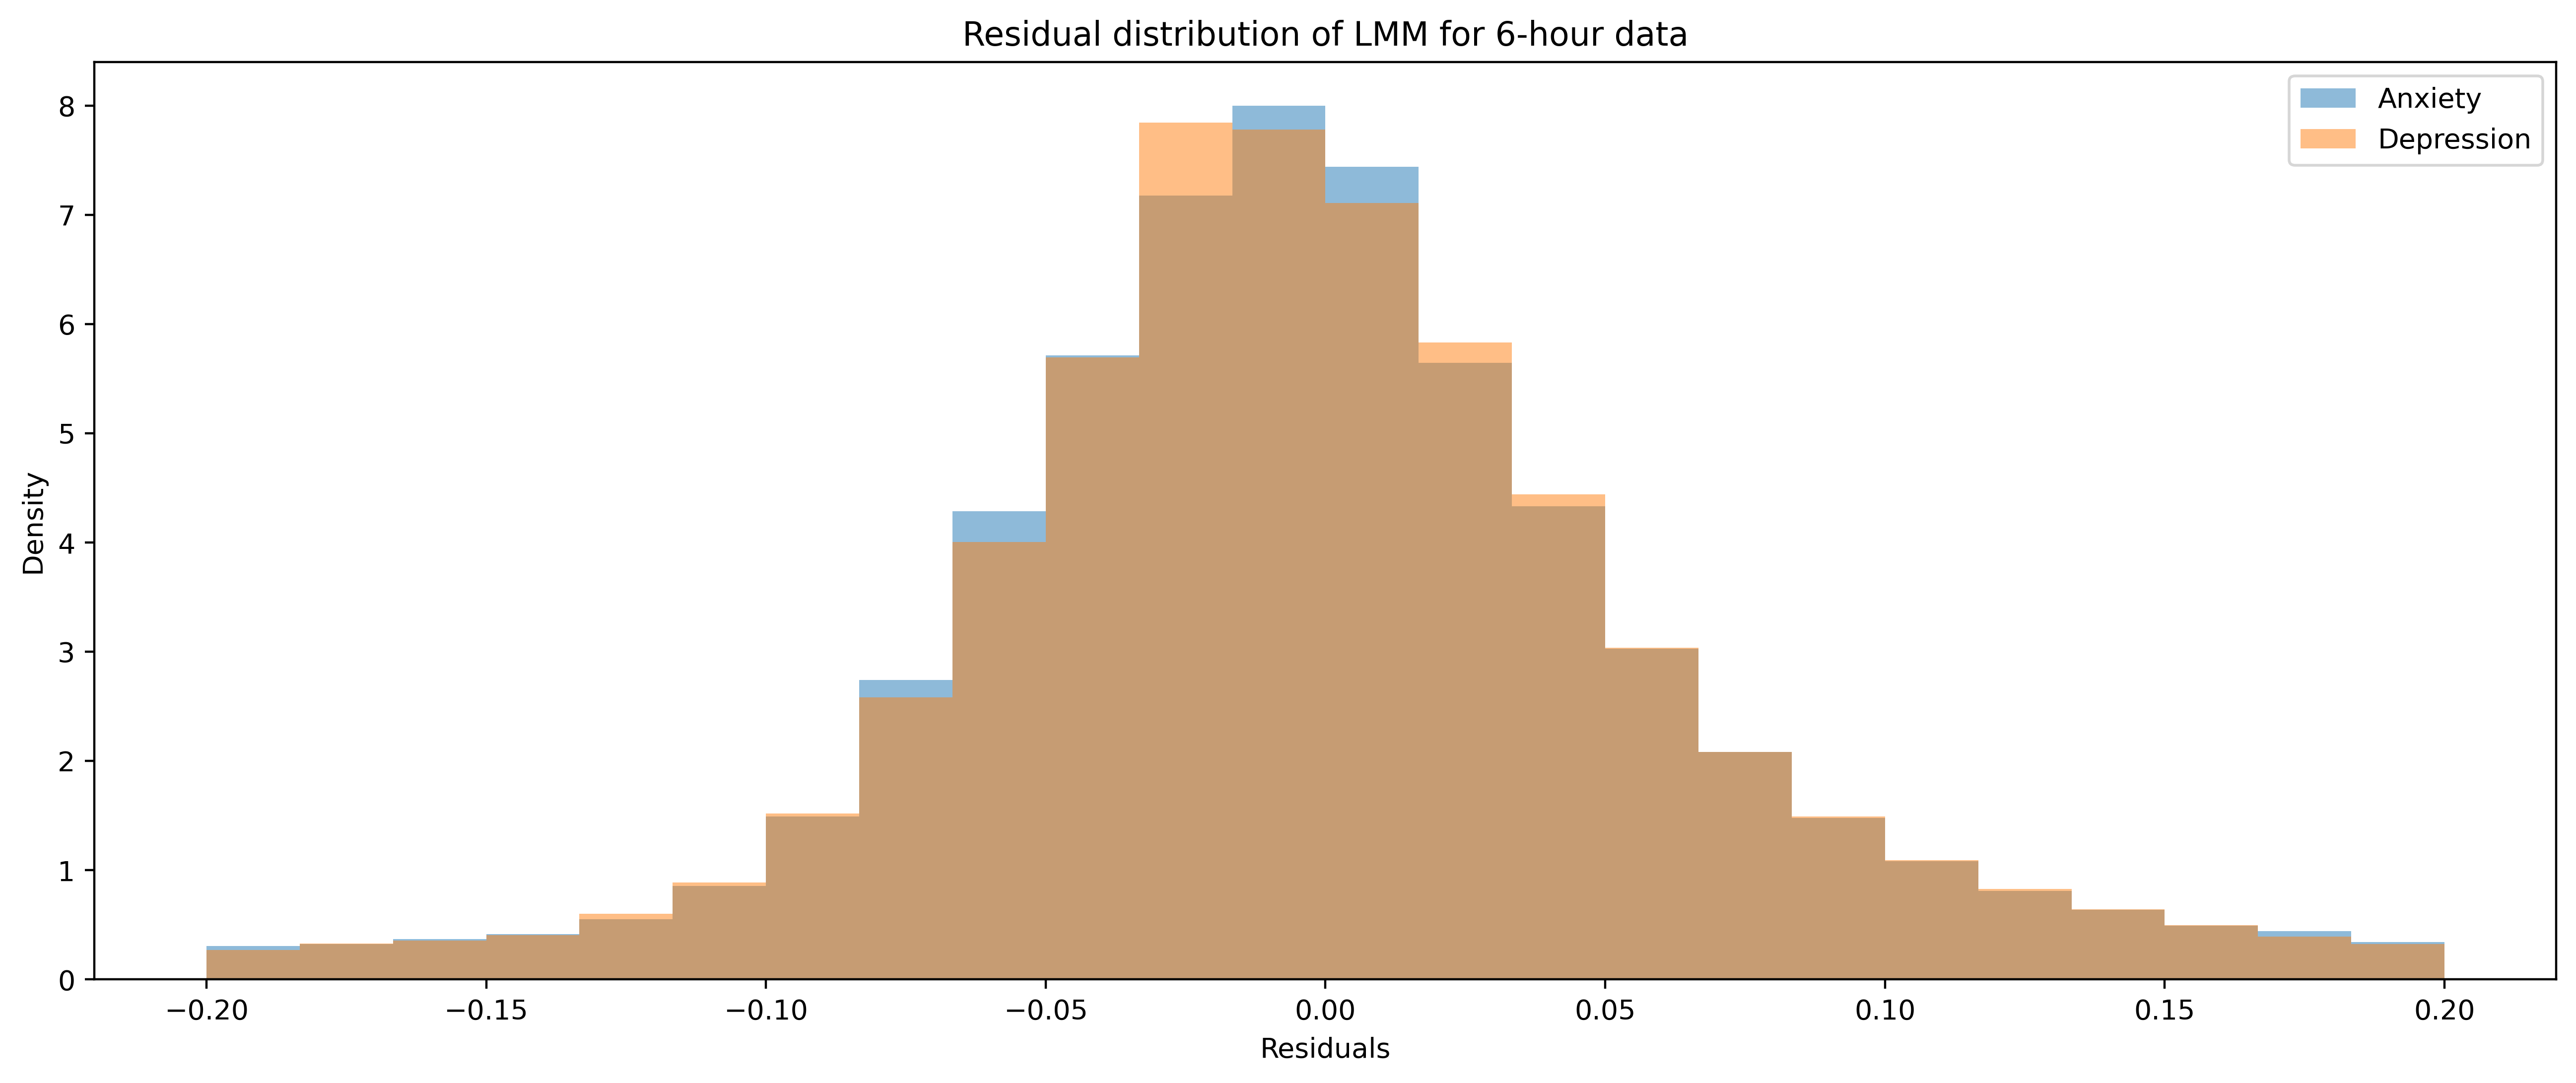
\includegraphics[width=\linewidth]{Images/lmm_6hr_roberta_residuals.png}
    \caption{Residual distribution for LMM predictions of 6-hour windowed RoBERTa NA scores.}
    \label{fig:roberta-lmm-residuals}
\end{figure}

The overall NA level was still significantly lower for the A cohort ($B = -0.0059; p = .04$), supporting earlier findings.

%TBD: This is counter-intuitive, but 
%it might be that our covariates dont fit anxiety patients
%otherwise interesting finding that anxiety patients appear to have higher NA variability
%future work: re-run the roberta analysis with all tweets

%Taken together, these findings suggest that — in the absence of temporal aggregation or smoothing — the transformer-based sentiment analysis does not capture statistically robust differences in either NA levels or NA variability between anxiety and depression groups, despite small descriptive differences pointing in the expected direction (see Figure \ref{fig:roberta_na_dist}. This further underscores the potential importance of modeling approach when attempting to extract NA information from online user activity data.



\begin{figure}[h]
    \centering
    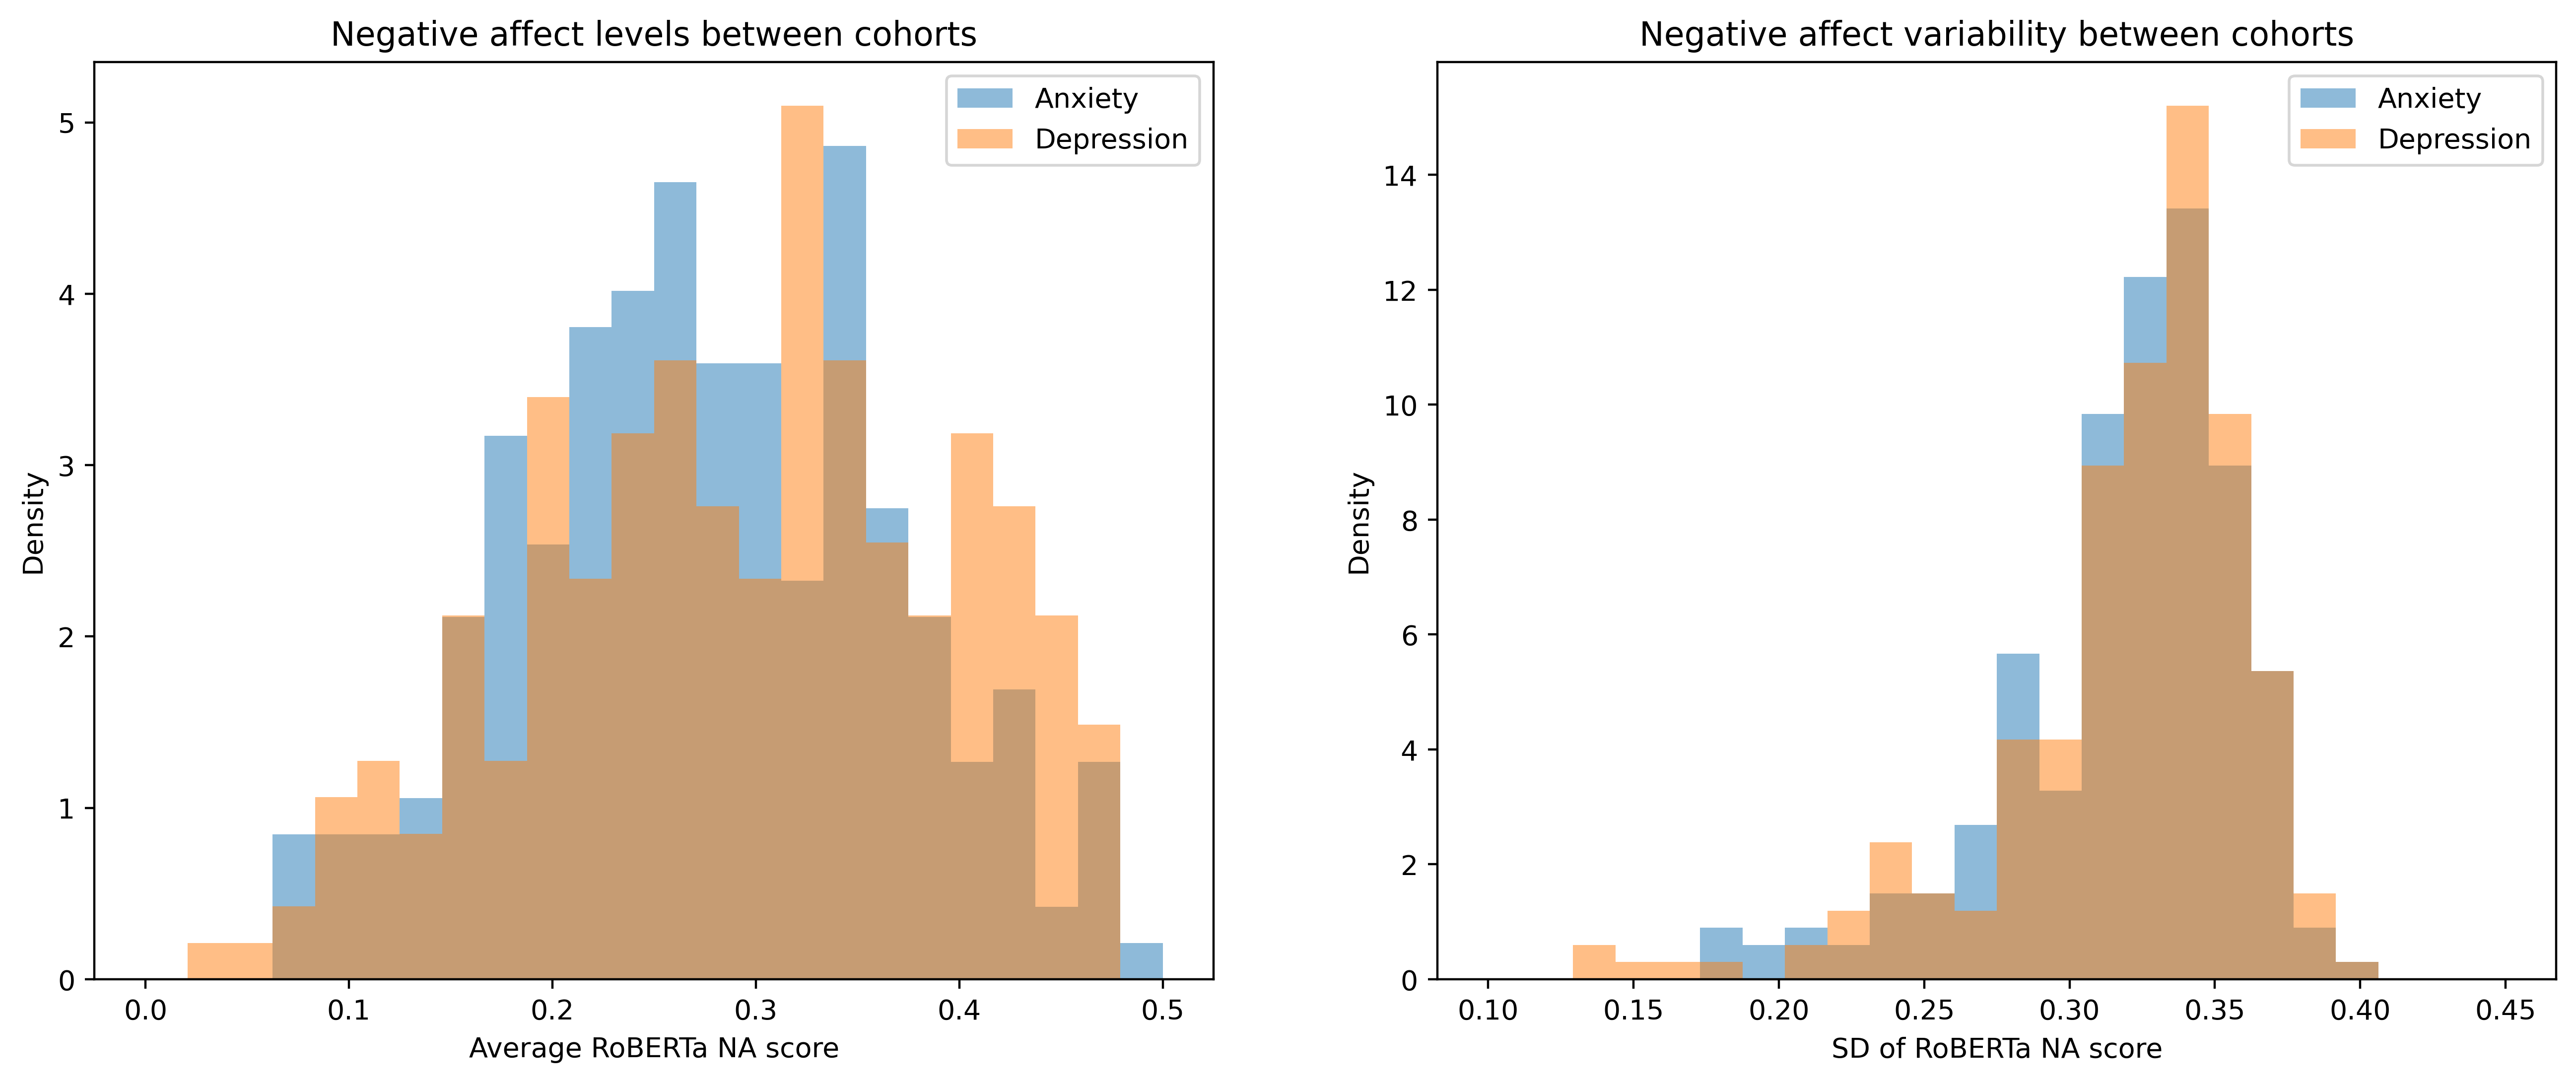
\includegraphics[width=\linewidth]{Images/na_histograms_raw_roberta.png}
    \caption{Means and standard deviations of RoBERTa NA scores across the entire time series.}
    \label{fig:roberta_na_dist}
\end{figure}



\subsubsection{Bounded distributions}

The paired sub-samples of the D and A cohorts showed to have highly similar mean VADER NA scores across the time series ($\bar{x}_D = 0.084883, \bar{x}_A = 0.084881$). The D cohort had a larger standard deviation with $\sigma^2_D = 0.134322$, while the A cohort had $\sigma^2_A = 0.130531$ (see Figure \ref{fig:bounded_boxes}).

This difference in standard deviation was statistically significant as shown by paired t-test ($t(647) = 4.86; p < .001$), indicating that the A cohort showed significantly lower NA variability than the D cohort, even when controlling for differences in overall NA levels.

\begin{figure}[h]
    \centering
    
\includegraphics[width=\linewidth]{Images/boxplot_depression_anxiety.png}
    \caption{Standard deviation and mean VADER NA score of paired sub-samples.}
    \label{fig:bounded_boxes}
\end{figure}

For the same analysis, but based on the RoBERTa sentiment estimations, a significant difference in NA variability between the cohorts also emerged. In this, case, it pointed to the opposite direction though. The A cohort had a larger standard deviation at $\sigma^2_A = 0.3248$, as opposed to $\sigma^2_D = 0.3215$ for the D cohort. The result was statistically significant ($t(183) = -2.19; p = .03$).

Thus, this indicates that anxiety patients actually showed higher NA variability than depression patients when comparing RoBERTa scores.


\begin{figure}[h]
    \centering
    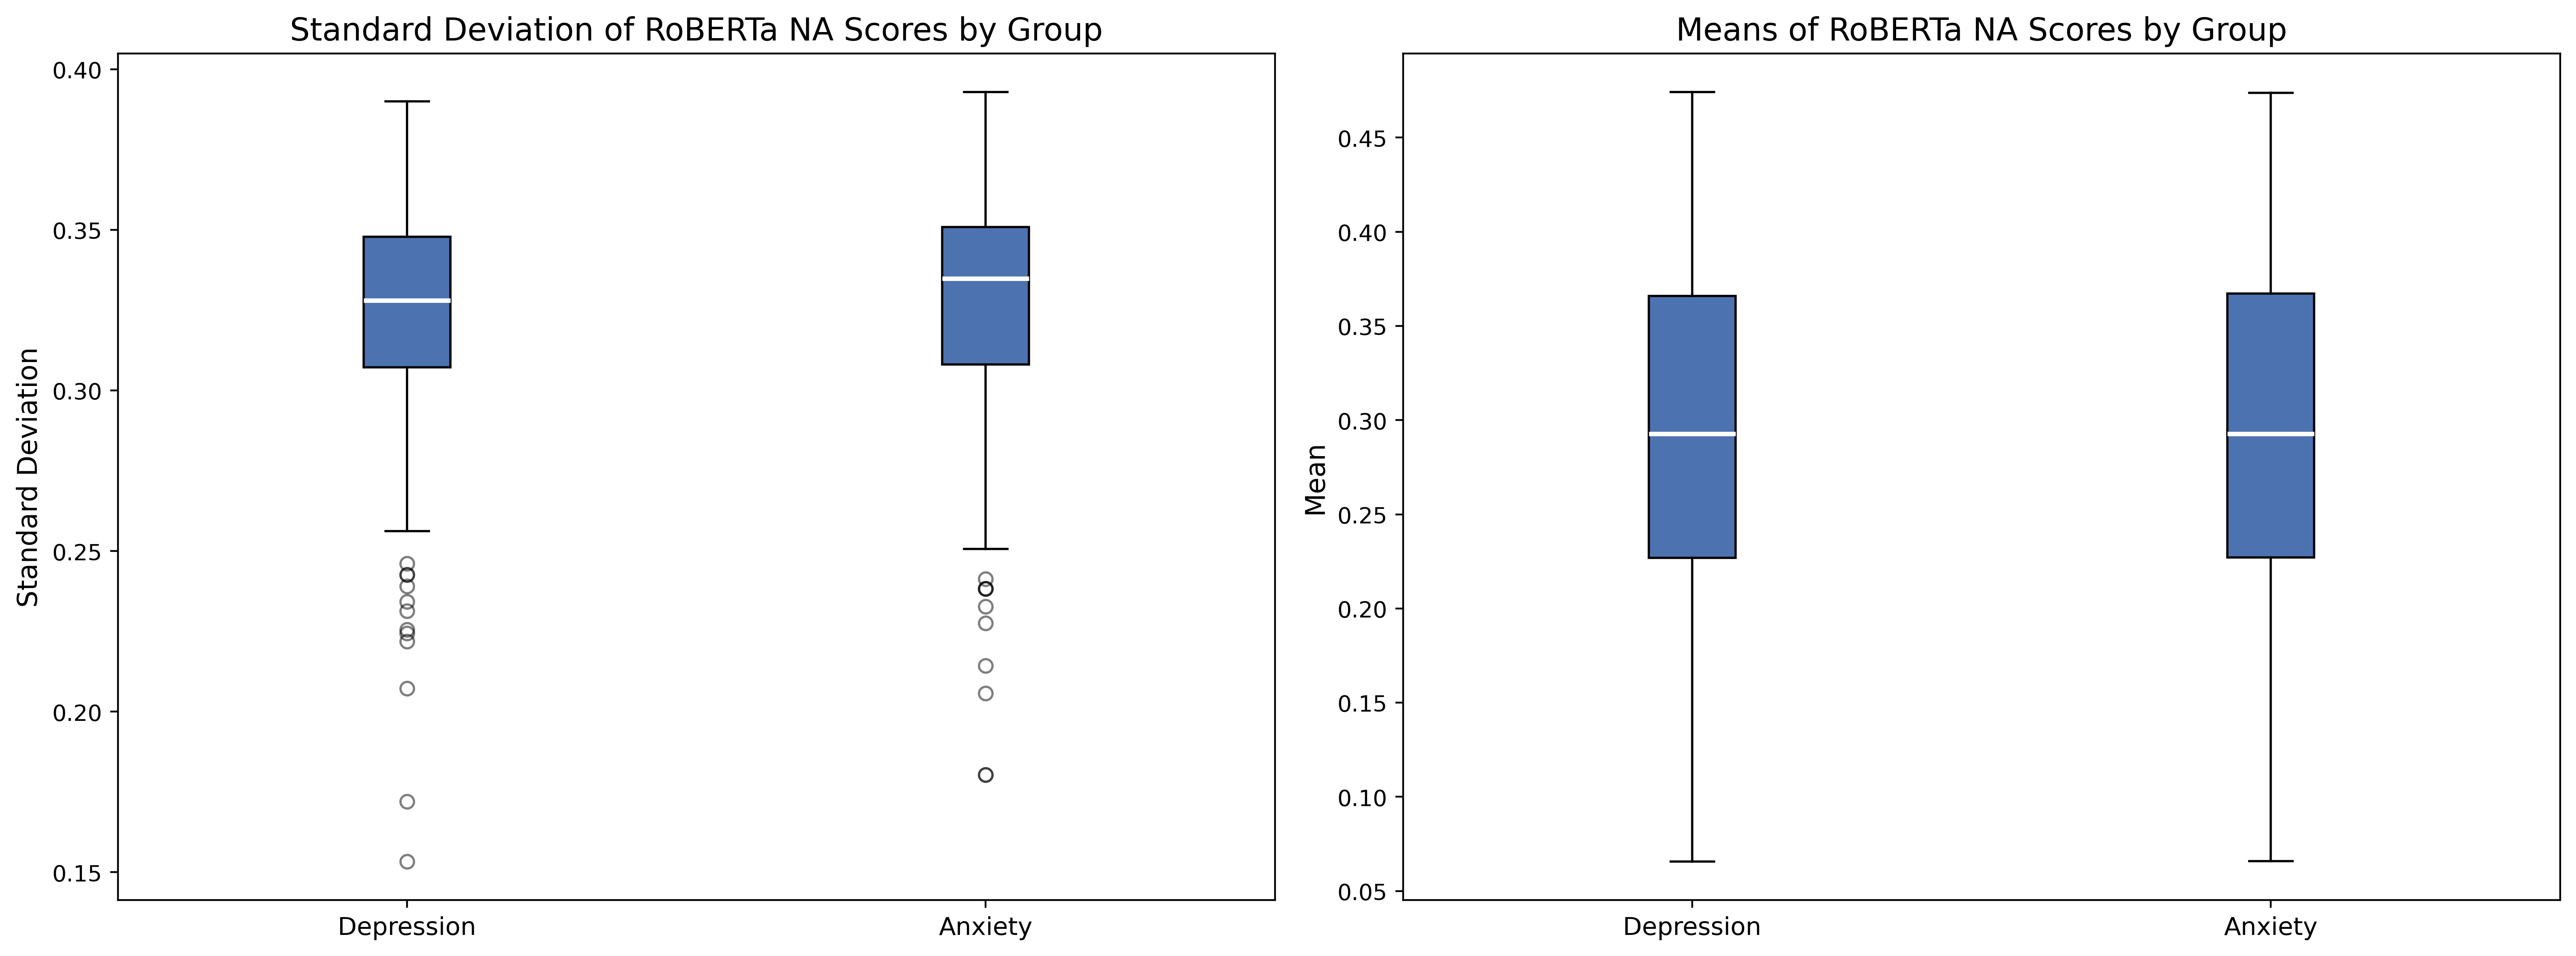
\includegraphics[width=\linewidth]{Images/boxplot_depression_anxiety_roberta.png}
    \caption{Standard deviation and mean RoBERTa NA score of paired sub-samples.}
    \label{fig:bounded_boxes}
\end{figure}

%\subsubsection{Notes...}
%- LMM
%    - If the previous tweet was more than an hour ago, it becomes much more %difficult to predict NA level
%    - results also remain for just checking tweets that had another recently
%- LMM based sentiments